\section{Описание практической части}
\label{sec:Chapter4} \index{Chapter4}
\subsection{Описание выбранного инструментария}
Работа была написана на языке Python, основной фреймворк для сбора данных -- Scrapy, так как эта библиотека позволяет
гибко настраивать параметры запросов, их обработку, генерацию cookie-файлов, поддерживает множественные подключения к ресурсы, 
асинхронно собирает данные \cite{scrapyBook}. В качестве базы данных
выступает MongoDB, поскольку она хранит данные в формате JSON-подобных документов \cite{mongoDBBook}. 

\par
Поскольку поиск в поисковых сервисах и поиск в социальной сети LinkedIn отличается по концепции и настройке пауков Scrapy, то
они были выделены в 2 различных проекта.

\subsubsection{Архитектура работы сборщиков в поисковых сервисах}
\par
Диаграмма классов приведена на рис. 7.

\begin{figure}[H]
    \center{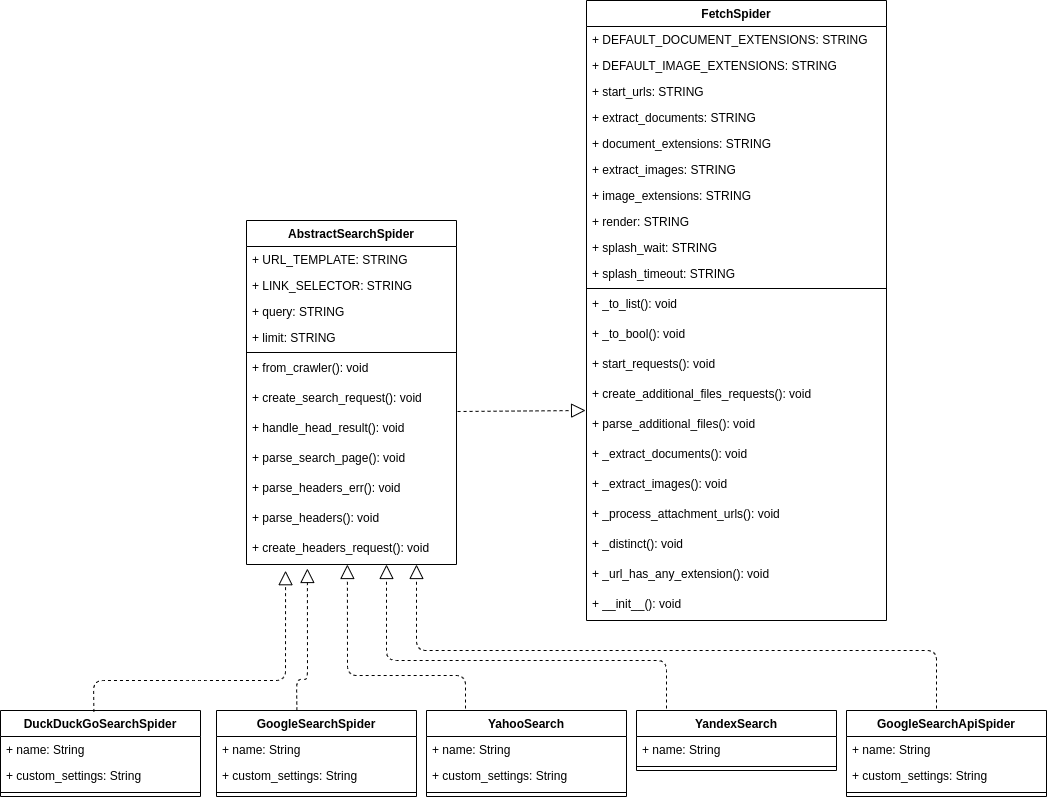
\includegraphics[height=10cm,keepaspectratio]{pictures/SearchNews.png}}
    \caption{Диаграмма классов сборщик в поисковых сервисах.}
    \label{ris:image}
\end{figure}

Система включает следующие 9 классов:
\begin{itemize}
    \item Сборщики данных:
    \begin{itemize}
        \item FetchSpider -- позволяет собирать все документы, изображения и html-код страницы;  
        \item AbstractSearchSpider -- содержит общие метода генерации запросов, обхода страниц и сбора данных с них;
        \item DuckDuckGoSearchSpider -- реализует конструктор запуска сборщика для поискового сервиса DuckDuckGo и несколько 
        специфичных констант, таких как шаблон url с query и CSS-селектор найденных ссылок;
        \item GoogleSearchSpider -- реализует конструктор запуска сборщика для поискового сервиса Google и несколько 
        специфичных констант, таких как шаблон url с query и CSS-селектор найденных ссылок;
        \item YahooSearch -- реализует конструктор запуска сборщика для поискового сервиса Yahoo и несколько 
        специфичных констант, таких как шаблон url с query и CSS-селектор найденных ссылок;
        \item YandexSearch -- реализует конструктор запуска сборщика для поискового сервиса Yandex и несколько 
        специфичных констант, таких как шаблон url с query и CSS-селектор найденных ссылок, настройки прокси;
        \item GoogleSearchApiSpider -- реализует сборщик для поискового сервиса Google, который будет
        производить сбор с помощью Google API Search.
    \end{itemize}
    \item Вспомогательные классы:
    \begin{itemize}
        \item GoogleAPICredentialsDownloaderMiddleware -- данный класс производит неким проводником между Scrapy Engine и 
        GoogleSearchApiSpider, в нем идет выбор API-ключа по стратегии <<выбери тот ключ, у которого осталось 
        наибольшее количество запросов>> и обработка 429 ошибки (случай, когда API-ключ неожиданно превысил лимит 
        использований и его необходимо признать невалидным, и запустить запрос с новым ключом);
        \item SplashFilesPipeline -- выкачивает все файлы, которые были получены в ходе сбора, если отобранная 
        ссылка была ссылкой не на html-страницу. 
    \end{itemize}
\end{itemize}


\subsubsection{Архитектура работы сборщиков в социальной сети LinkedIn}


Система включает следующие n классов:
\begin{itemize}
    \item поиск и сбор с помощью навигации по атрибутам html-кода страницы и извлечение информации из атрибутов:
    \begin{figure}[H]
        \center{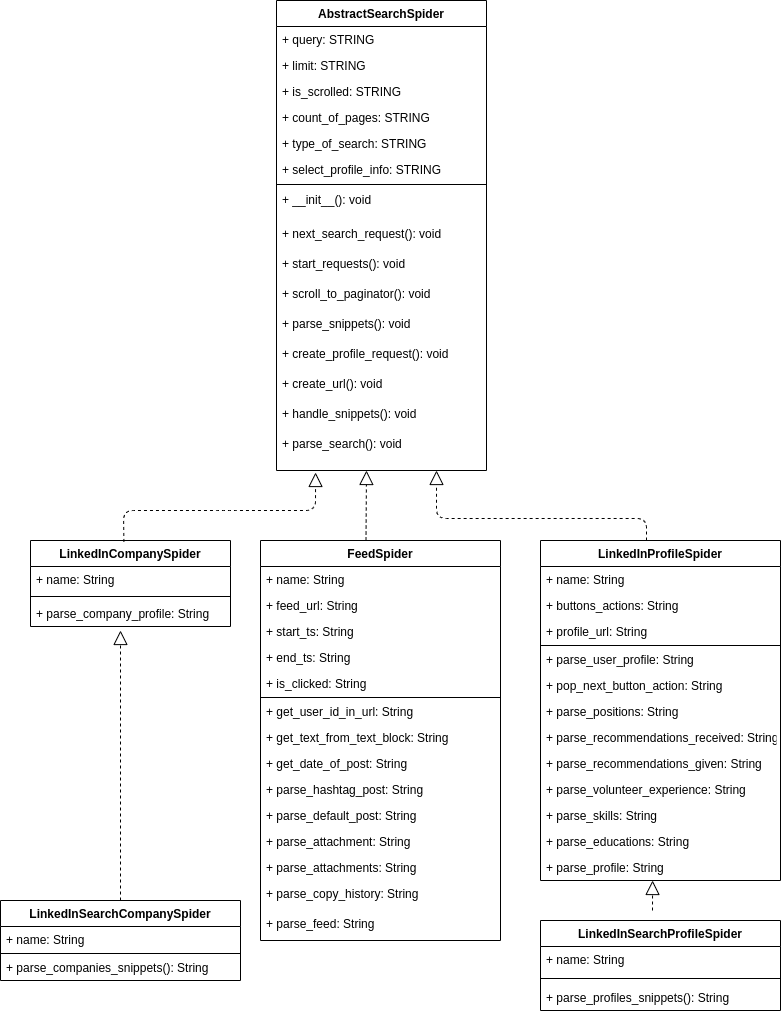
\includegraphics[height=14cm,keepaspectratio]{pictures/LinkedInWeb.png}}
        \caption{Диаграмма классов сборщик в социальной сети LinkedIn web.}
        \label{ris:image}
    \end{figure}
    \begin{itemize}
        \item AbstractSearchSpider -- абстрактный класс для поиска и сбора людей и организаций;
        \item LinkedInCompanySpider -- сборщик данных компаний;
        \item FeedSpider -- сбор данных новостной ленты пользователя; 
        \item LinkedInProfileSpider -- сборщик данных пользователей;
        \item LinkedInSearchCompanySpider -- поисковик компаний внутри социальной сети. При настройке имеет возможность 
        собирать информацию о найденных организациях;
        \item LinkedInSearchProfileSpider -- поисковик пользователей внутри социальной сети. При настройке имеет возможность
        собирать информацию о найденных людях.
    \end{itemize}
    \item поиск и сбор с помощью закрытого LinkedIn API:
    \begin{figure}[H]
        \center{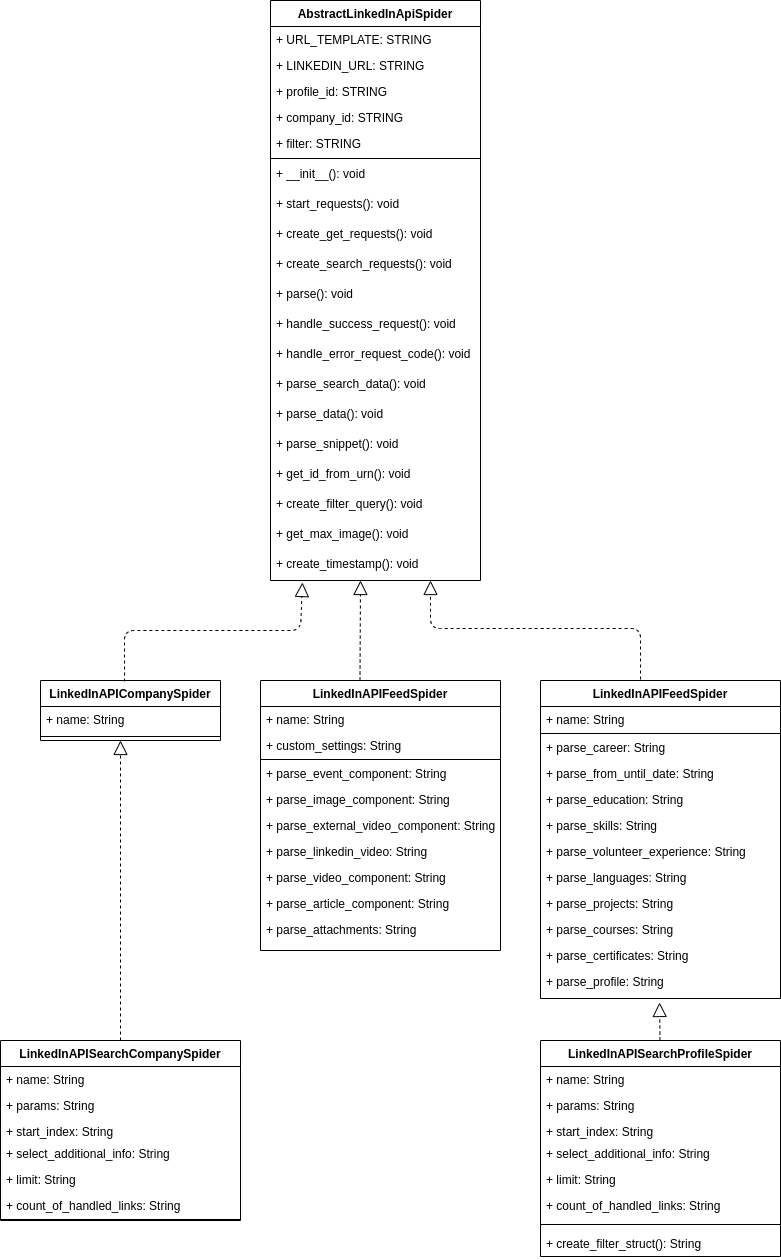
\includegraphics[height=14cm,keepaspectratio]{pictures/LinkedInAPI.png}}
        \caption{Диаграмма классов сборщик в социальной сети LinkedIn API.}
        \label{ris:image}
    \end{figure}
    \begin{itemize}
        \item AbstractLinkedInApiSpider -- класс, который эмулирует для получения данных из социальной сети посредством
        API;
        \item LinkedInAPICompanySpider -- сборщик данных заданной компании;
        \item LinkedInAPIFeedSpider -- сборщик новостной ленты;
        \item LinkedInAPIProfileSpider -- сборщик данных заданного пользователя;
        \item LinkedInAPISearchProfileSpider -- производит поиск пользователей по заданным фильтрам. Имеет возможность 
        собирать информацию о найденных людях при настройке;
        \item LinkedInAPISearchCompanySpider -- производит поиск компаний по заданным фильтрам. Имеет возможность 
        собирать информацию о найденных организациях при настройке.
    \end{itemize}
    \item Вспомогательные классы:
    \begin{itemize}
        \item AccountStatus -- перечисление со статусом аккаунта, под которым мы пытаемся собирать информацию в социальной
        сети;
        \item LinkedInCredentialsDownloaderMiddleware -- если в приложении нет cookie файлов или имеются устаревшие cookie, 
        данный класс перелогинивает указанный в настройках аккаунт при помощи GET и POST запросов в LinkedIn API. На выходе
        получаем обновленные cookie файлы и возможность дальше собирать информацию из социальной сети. 
    \end{itemize}  
\end{itemize}